\documentclass[paper=a4, fontsize=11pt]{scrartcl}
\usepackage[T1]{fontenc}
\usepackage{fourier}

\usepackage[english]{babel}															% English language/hyphenation
\usepackage[protrusion=true,expansion=true]{microtype}	
\usepackage{amsmath,amsfonts,amsthm} % Math packages
\usepackage[pdftex]{graphicx}	
\usepackage{url}
\usepackage{hyperref}


%%% Custom sectioning
\usepackage{sectsty}
\allsectionsfont{\centering \normalfont\scshape}
\usepackage{subfigure}


%%% Custom headers/footers (fancyhdr package)
\usepackage{fancyhdr}
\pagestyle{fancyplain}
\fancyhead{}											% No page header
\fancyfoot[L]{}											% Empty 
\fancyfoot[C]{}											% Empty
\fancyfoot[R]{\thepage}									% Pagenumbering
\renewcommand{\headrulewidth}{0pt}			% Remove header underlines
\renewcommand{\footrulewidth}{0pt}				% Remove footer underlines
\setlength{\headheight}{13.6pt}


%%% Equation and float numbering
\numberwithin{equation}{section}		% Equationnumbering: section.eq#
\numberwithin{figure}{section}			% Figurenumbering: section.fig#
%\numberwithin{table}{section}				% Tablenumbering: section.tab#


%%% Maketitle metadata
\newcommand{\horrule}[1]{\rule{\linewidth}{#1}} 	% Horizontal rule

\title{
		%\vspace{-1in} 	
		\usefont{OT1}{bch}{b}{n}
		\normalfont \normalsize \textsc{CS650 - Computer Vision} \\ [25pt]
		\horrule{0.5pt} \\[0.4cm]
		\huge Programming Lab 2 \\ Edge Detection / Hough Transform \\
		\horrule{2pt} \\[0.5cm]
}
\author{
		\normalfont 								\normalsize
        Daqing Yi\\[-3pt]		\normalsize
        \today
}
\date{}


%%% Begin document
\begin{document}
\maketitle

Prepare a brief writeup that includes each part and submit it as a PDF through Canvas.
Your writeup should document your findings for Part 1 but otherwise focus on your methods and results for Part 2.

Note: many of the images for Part 1 will contain negative numbers or numbers larger than 255.
Make sure you appropriately scale the output images to display all of the information.
(Hint: if there are negative values, try mapping 0 to 128 with positive values mapped to the range (128,255] and negative values to the range [0,128).]

This lab consists of two parts, binarization and morphology.
The implementations are written in Python.
PIL is used for reading image files into data arrays.
Numpy is used for array operations.
Matplotlib is used for visualizing data.
Open CV is used to verify the correctness.

\section{Edge detection}

\subsection{First and Second Order Derivatives of an Image}

\begin{figure}[h]
\centering
\subfigure[Origin]{
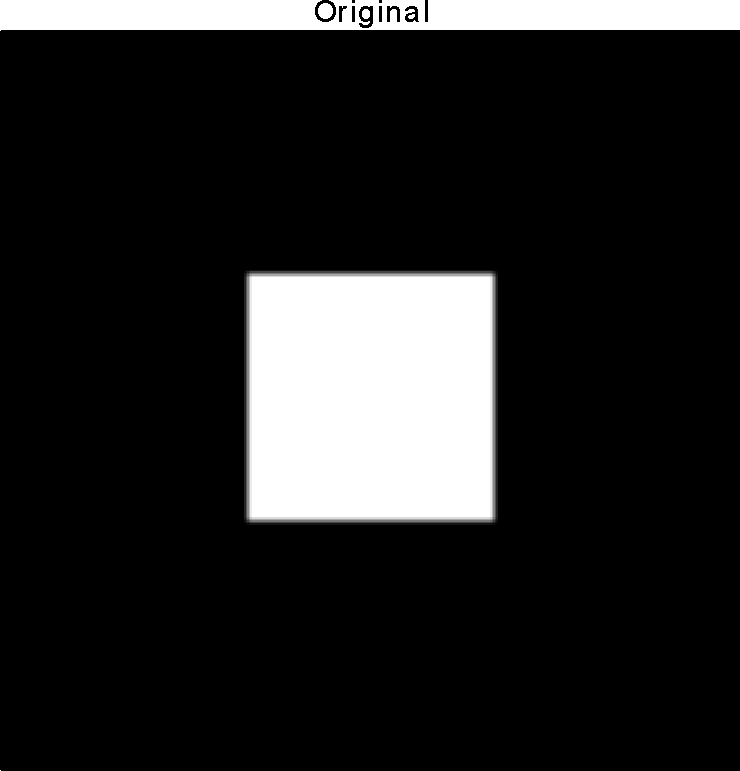
\includegraphics[width=.23\textwidth]{./figure/2D_White_Box_origin}
\label{fig:edge:01:origin} }
\subfigure[Gradient Magnitude]{
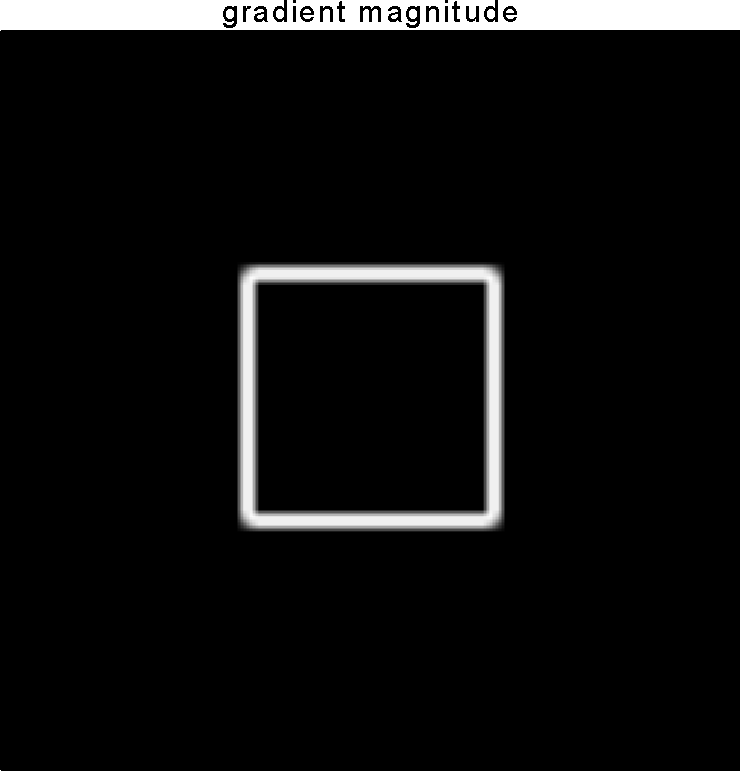
\includegraphics[width=.23\textwidth]{./figure/2D_White_Box_gradient_magnitude} 
\label{fig:edge:01:gradient_magnitude} }
\subfigure[Gradient Orientation]{
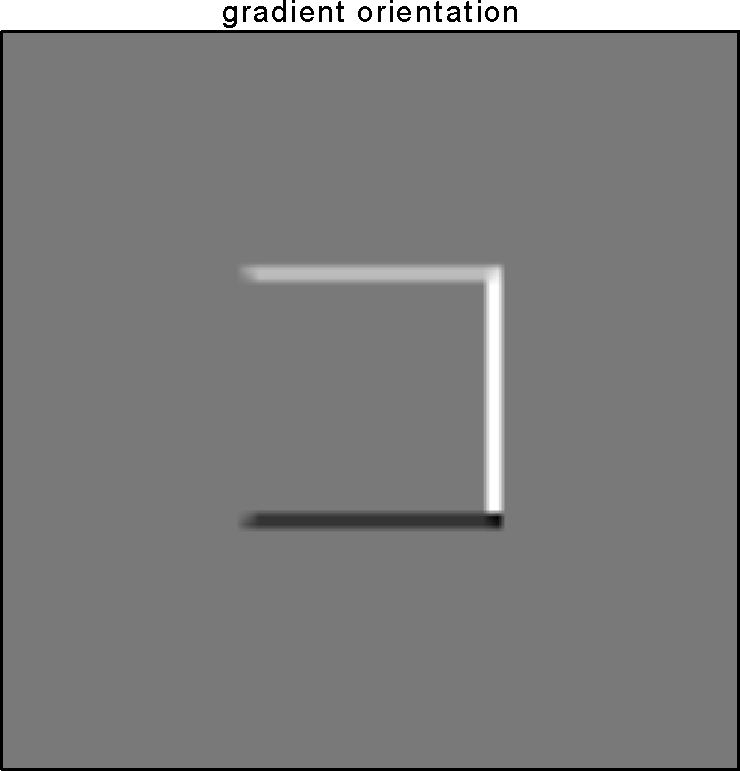
\includegraphics[width=.23\textwidth]{./figure/2D_White_Box_gradient_orientation}
\label{fig:edge:01:gradient_orientation} }
\subfigure[Laplacian]{
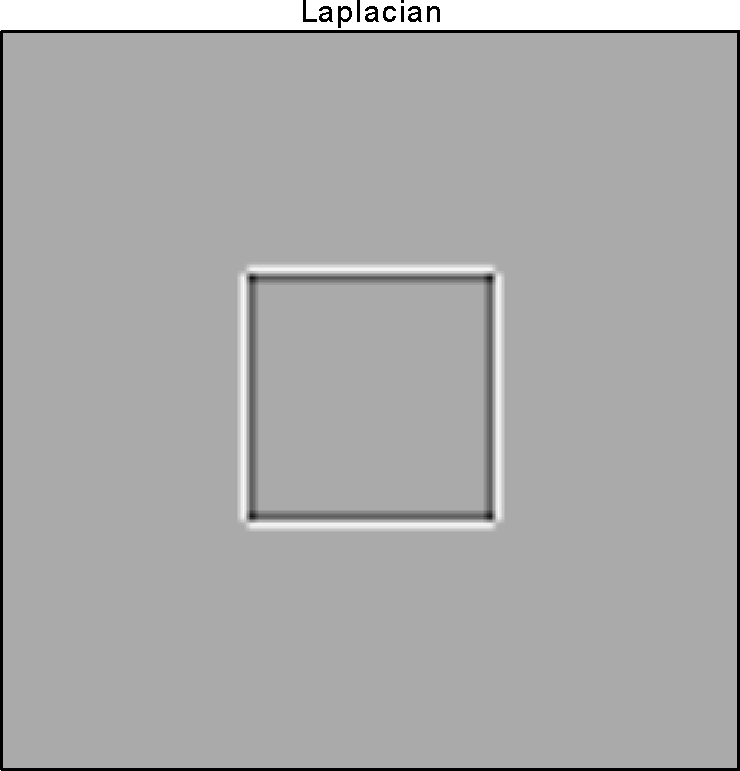
\includegraphics[width=.23\textwidth]{./figure/2D_White_Box_laplacian} 
\label{fig:edge:01:laplacian} }
\caption{Derivatives of \emph{2D\_White\_Box.pgm} by 1st order and 2nd order.}
\label{fig:edge:01}
\end{figure}

\begin{figure}[h]
\centering
\subfigure[Origin]{
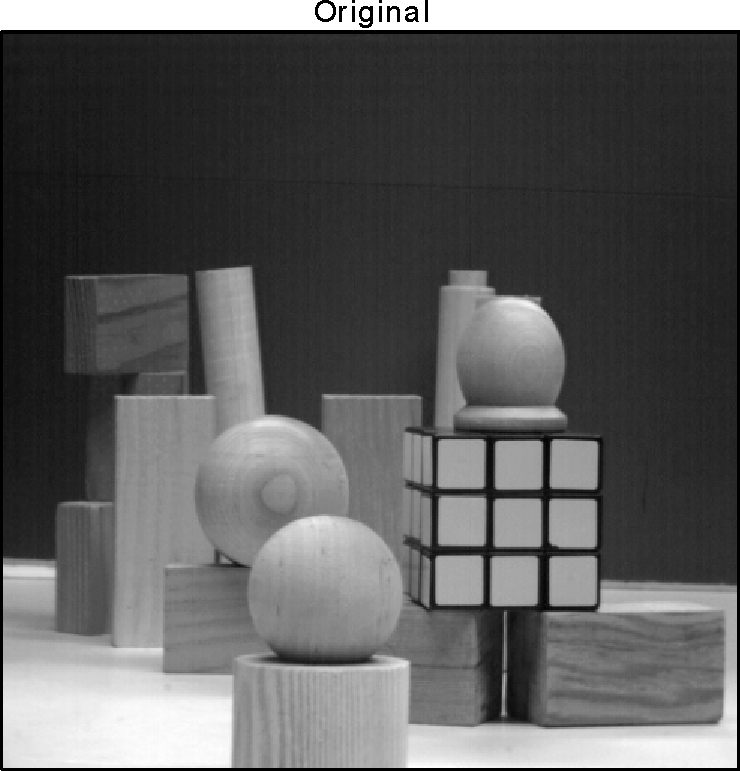
\includegraphics[width=.47\textwidth]{./figure/blocks_origin}
\label{fig:edge:02:origin} }
\subfigure[Gradient Magnitude]{
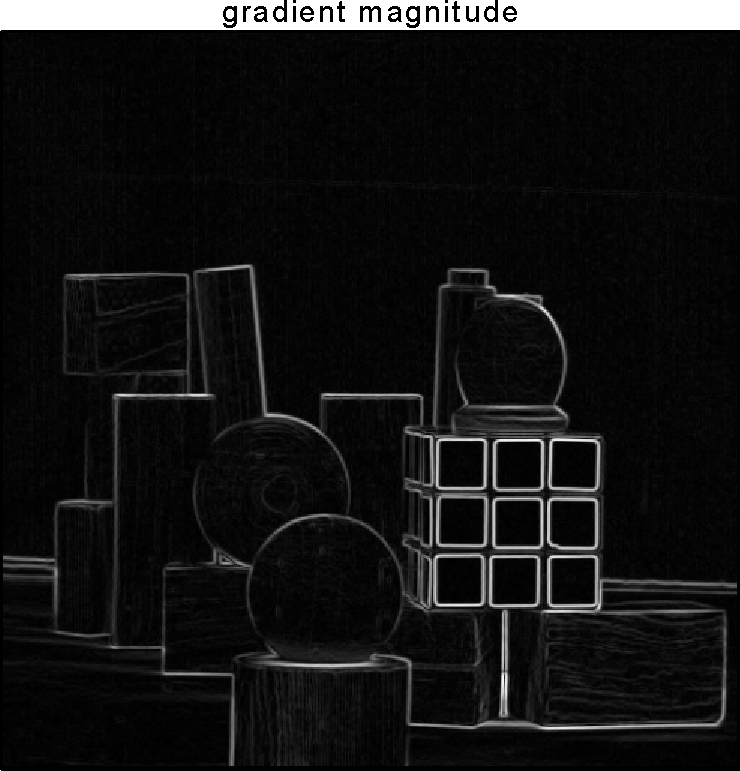
\includegraphics[width=.47\textwidth]{./figure/blocks_gradient_magnitude} 
\label{fig:edge:02:gradient_magnitude} } \\
\subfigure[Gradient Orientation]{
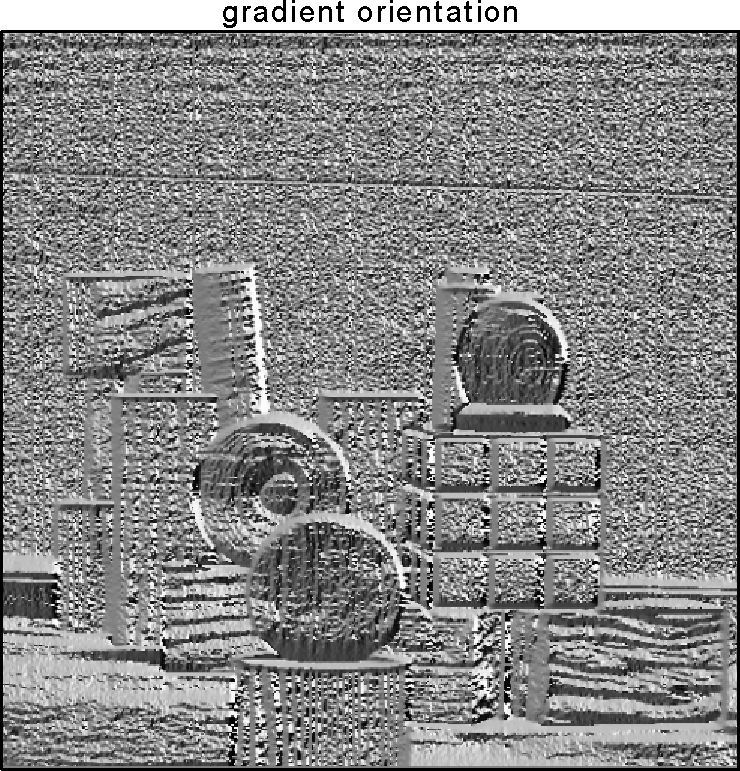
\includegraphics[width=.47\textwidth]{./figure/blocks_gradient_orientation}
\label{fig:edge:02:gradient_orientation} }
\subfigure[Laplacian]{
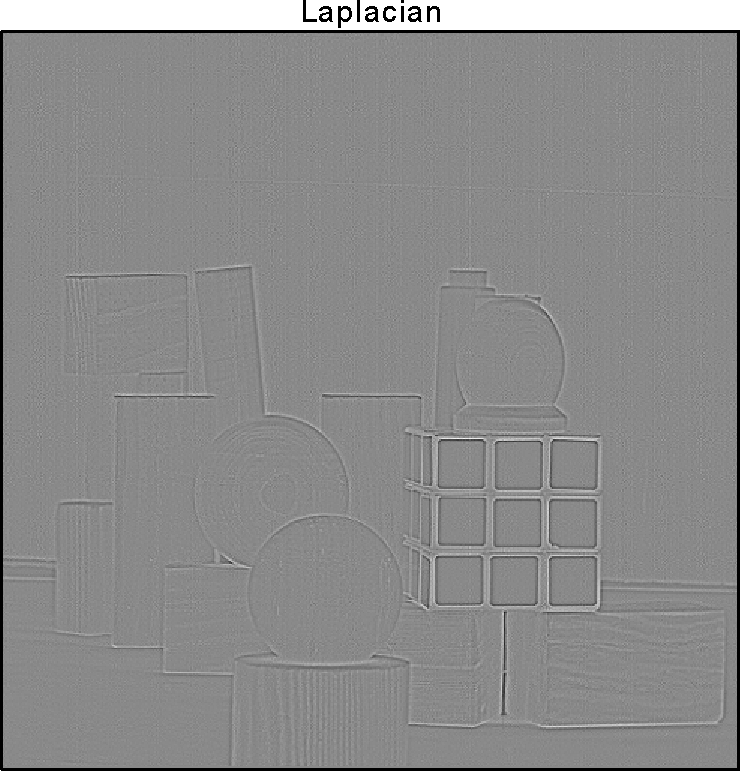
\includegraphics[width=.47\textwidth]{./figure/blocks_laplacian} 
\label{fig:edge:02:laplacian} }
\caption{Derivatives of \emph{blocks.pgm} by 1st order and 2nd order.}
\label{fig:edge:02}
\end{figure}

\subsection{edge detection}

\subsubsection{Canny edge detector}

\begin{figure}[h]
\centering
\subfigure[hi\_thresh=40, lo\_thresho=20]{
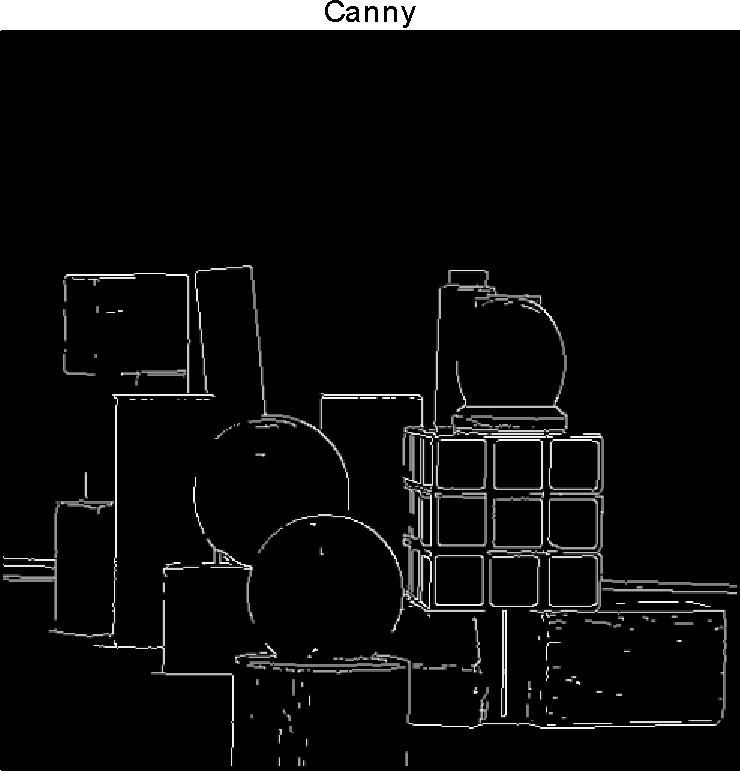
\includegraphics[width=.235\textwidth]{./figure/blocks_canny_20_40}
\label{fig:edge:02:canny:1} }
\subfigure[hi\_thresh=60, lo\_thresho=30]{
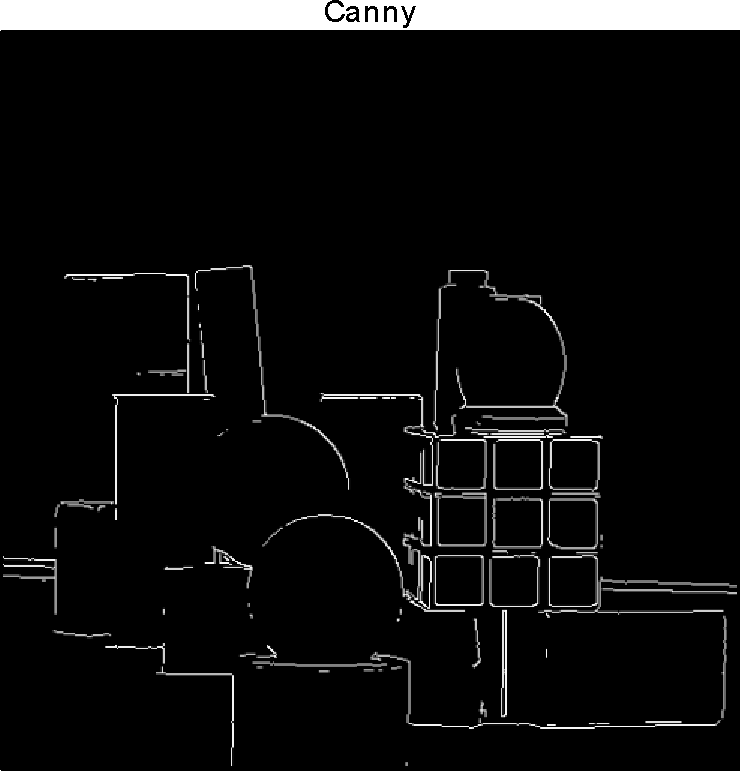
\includegraphics[width=.235\textwidth]{./figure/blocks_canny_30_60} 
\label{fig:edge:02:canny:2} } 
\subfigure[hi\_thresh=80, lo\_thresho=40]{
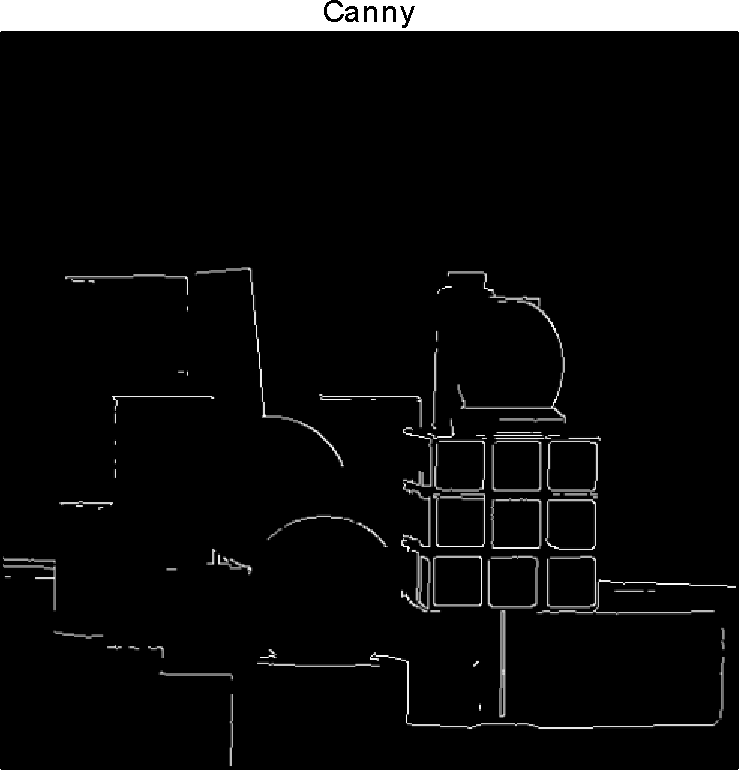
\includegraphics[width=.235\textwidth]{./figure/blocks_canny_40_80}
\label{fig:edge:02:canny:3} }
\subfigure[hi\_thresh=60, lo\_thresho=30, with Gaussian filter]{
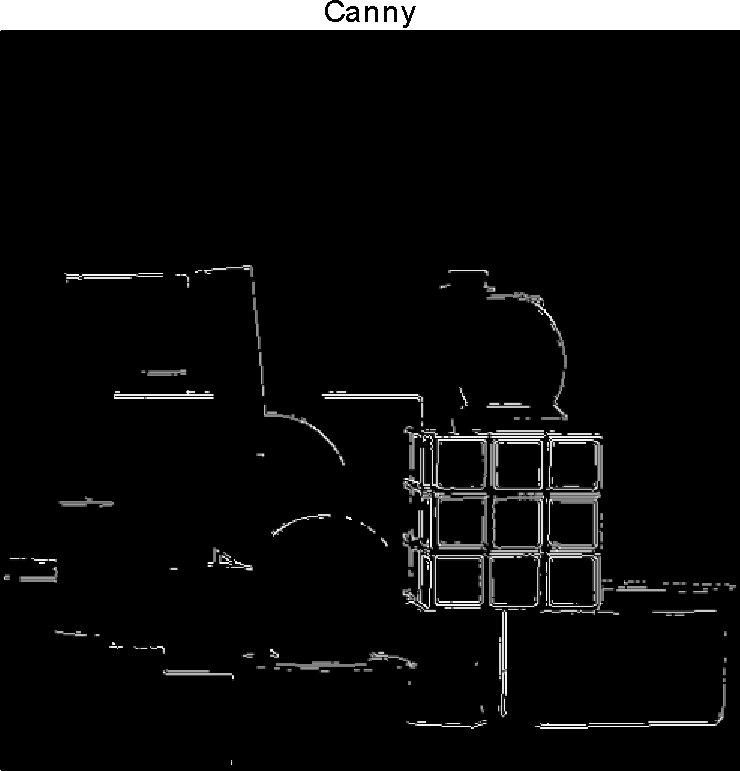
\includegraphics[width=.235\textwidth]{./figure/blocks_canny_gauss_30_60} 
\label{fig:edge:02:canny:gauss} }
\caption{Canny edge detector on \emph{blocks.pgm} using different parameters.}
\label{fig:edge:02:canny}
\end{figure}

\subsection{Laplacian zero-crossing edge detector}

\begin{figure}[h]
\centering
\subfigure[Threshold=40]{
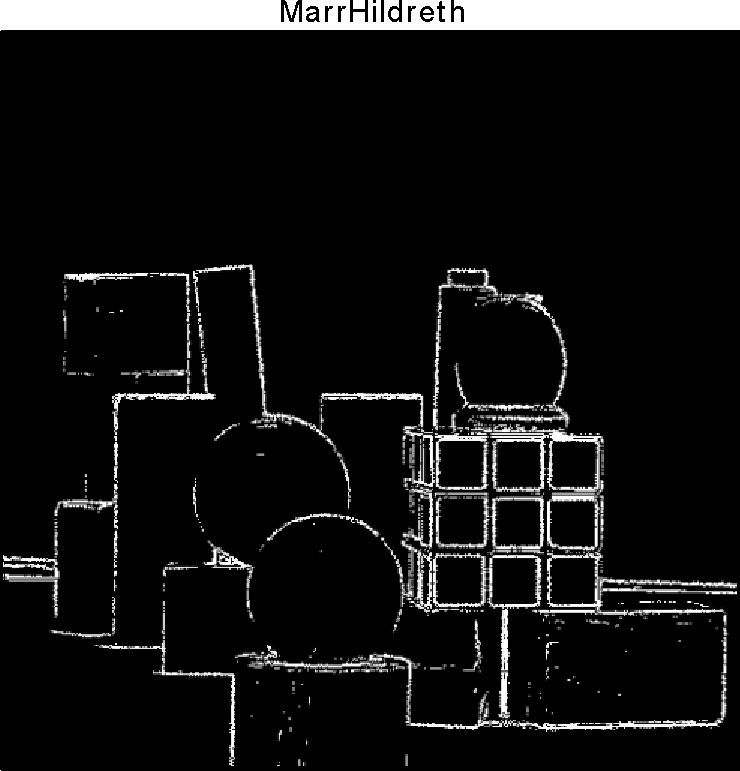
\includegraphics[width=.235\textwidth]{./figure/blocks_mh_40}
\label{fig:edge:02:mh:1} }
\subfigure[Threshold=60]{
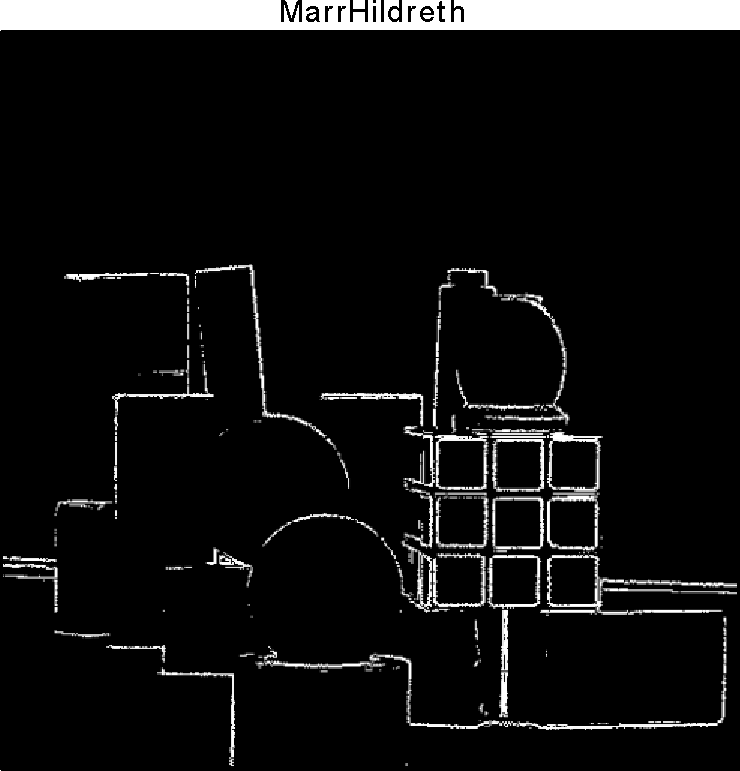
\includegraphics[width=.235\textwidth]{./figure/blocks_mh_60} 
\label{fig:edge:02:mh:2} } 
\subfigure[Threshold=80]{
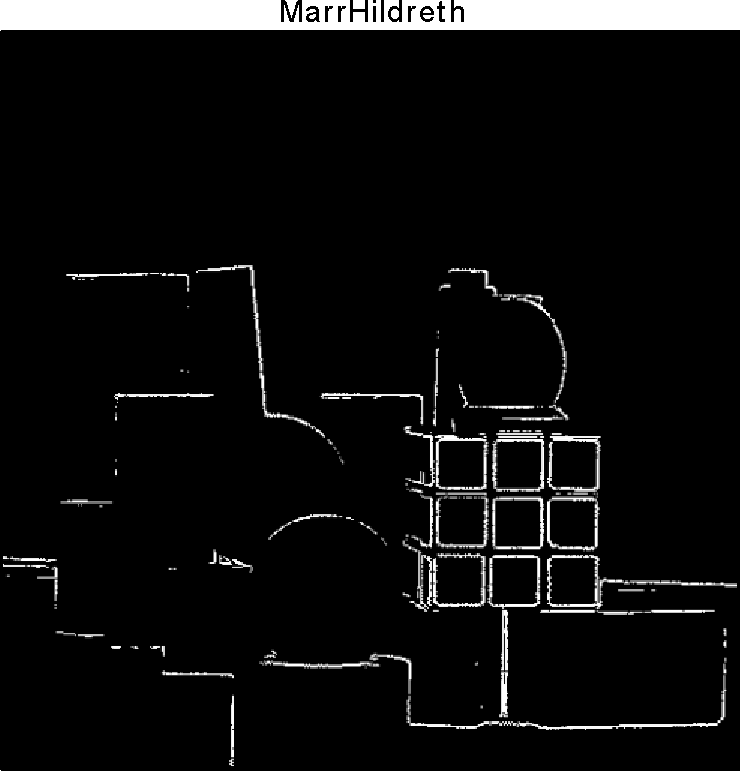
\includegraphics[width=.235\textwidth]{./figure/blocks_mh_80}
\label{fig:edge:02:mh:3} }
\subfigure[Threshold=40, with Gaussian filter]{
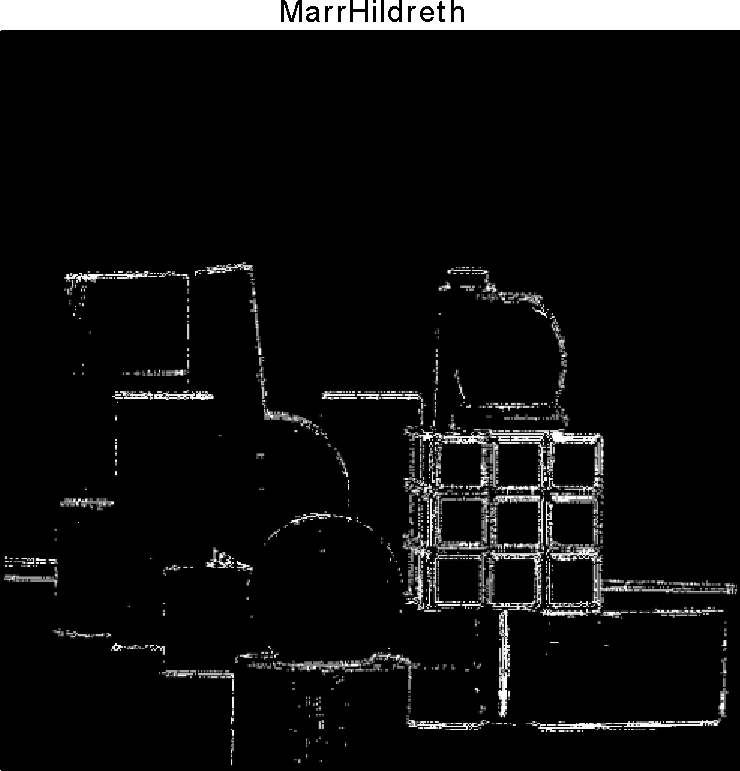
\includegraphics[width=.235\textwidth]{./figure/blocks_mh_gauss_40} 
\label{fig:edge:02:mh:gauss} }
\caption{Laplacian zero-crossing edge detector on \emph{blocks.pgm} using different parameters.}
\label{fig:edge:02:mh}
\end{figure}

\section{Hough transformation}

\subsection{Conclusion}



\end{document}